\documentclass{beamer}

\usetheme{CambridgeUS}
\usecolortheme{orchid}

\usepackage[utf8]{inputenc}
\usepackage[T1]{fontenc}

% Paths
\newcommand{\figs}{../figs}
\newcommand{\data}{../data}
\newcommand{\code}{../code}

% URL styles
\usepackage{url}
\urlstyle{sf}

% Units
\usepackage[detect-weight=true, binary-units=true]{siunitx}
\DeclareSIUnit\flop{Flops}

% Math
\usepackage{amsmath}
\usepackage{amssymb}
\usepackage{bm}
\usepackage{nicefrac}
\newcommand{\dif}[1]{{\;\text{d}#1}}

% Graphics
\usepackage{graphicx}
\usepackage{caption}
\usepackage{subcaption}
\graphicspath{{../figs/}}

% Tikz
\usepackage{tikz}
\usetikzlibrary{positioning,shapes,arrows,calc,intersections}
\usepackage{pgfplots}
\usepgfplotslibrary{dateplot}
\pgfplotsset{compat=1.8}

% Colors
\definecolor{darkblue}{HTML}{00688B}
\definecolor{darkgreen}{HTML}{6E8B3D}
\definecolor{cadet}{HTML}{DAE1FF}
\definecolor{salmon}{HTML}{FFB08A}

% Listings
\usepackage{textcomp}
\usepackage{listings}
\lstset{
  keywordstyle=\bfseries\color{orange},
  stringstyle=\color{darkblue!80},
  commentstyle=\color{darkblue!80},
  showstringspaces=false,
  basicstyle=\ttfamily,
  upquote=true,
}
\lstdefinestyle{fortran}{
  language=Fortran,
  morekeywords={for},
  deletekeywords={status},
}
\lstdefinestyle{c}{
  language=C,
  morekeywords={include},
}
\lstdefinestyle{glsl}{
  language=C,
  morekeywords={attribute, vec2, vec3, vec4, varying, uniform, mat2, mat3, mat4},
}
\lstdefinestyle{cuda}{
  language=C,
  morekeywords={__global__, __device__, __host__},
}
\lstdefinestyle{shell}{
  language=bash,
  morekeywords={mkdir, ssh, cmake},
}

% Double hlines
\usepackage{hhline}

% Misc
\usepackage{nth}

\subtitle{TMA4280---Introduction to Supercomputing}

\begin{document}


\title{Trends in supercomputing}
\author{Eivind Fonn}
\institute{SINTEF ICT / NTNU}
\date{December 2015}
\maketitle

\begin{frame}
  \frametitle{Top 500 systems}
  \begin{center}
    \begin{tikzpicture}
  \begin{axis}[
    date coordinates in=x,
    ymode=log,
    xticklabel=\year,
    xmin=1993-05-01,
    xmax=2015-10-01,
    width=0.8\textwidth,
    height=0.6\textwidth,
    ytick={1, 1000, 1000000, 1000000000},
    yticklabels={$\SI{1}{\giga\flop}$, $\SI{1}{\tera\flop}$, $\SI{1}{\peta\flop}$, $\SI{1}{\exa\flop}$},
    grid=major,
    legend style={at={(1,0)}, anchor=south east},
    legend cell align=left,
    ]
    \addplot[mark=o, mark size=1.3, draw=darkgreen, thick]
    table[x=date, y=sum, col sep=comma]
    {\data/performance-development.csv};
    \addplot[mark=o, mark size=1.3, draw=red, thick]
    table[x=date, y=high, col sep=comma]
    {\data/performance-development.csv};
    \addplot[mark=o, mark size=1.3, draw=magenta, thick]
    table[x=date, y=low, col sep=comma]
    {\data/performance-development.csv};
    \legend{Sum, Highest, Lowest};
  \end{axis}
\end{tikzpicture}

  \end{center}
\end{frame}

\begin{frame}
  \frametitle{Supercomputers at NTNU}
  A supercomputing center was established in 1986. \\~\\
  \begin{center}
    \scalebox{0.8}{
      \bgroup\def\arraystretch{1.2}
\begin{tabular}{llrlr}
  \hline
  Year & System & Processors & Type & $\SI{}{\giga\flop}$ \\
  \hhline{=====}
  1986--1992 & Cray X-MP & 2 & Vector & 0.5 \\
  1992--1996 & Cray Y-MP & 4 & Vector & 1.3\\
  1995--2003 & Cray J90     & 8 & Vector & 1.6 \\
  1992--1999 & Intel Paragon & 56 & MPP & 5.0\\
  1996--2003 & Cray T3E & 96 & MPP & 58\\
  2000--2001 & SGI O2 & 160 & ccNUMA & 100\\
  2001--2008 & SGI O3 & 898 & ccNUMA & 1000\\
  2006--2011 & IBM P5+ & 2976 & Distributed SMP & 23500\\
  2012--     & SGI Altix ICE X & 23040 & Distributed SMP & 497230 \\
  \hline
\end{tabular}
\egroup

    }
  \end{center}
\end{frame}

\begin{frame}
  \frametitle{Previous supercomputer at NTNU}
  \begin{center}
    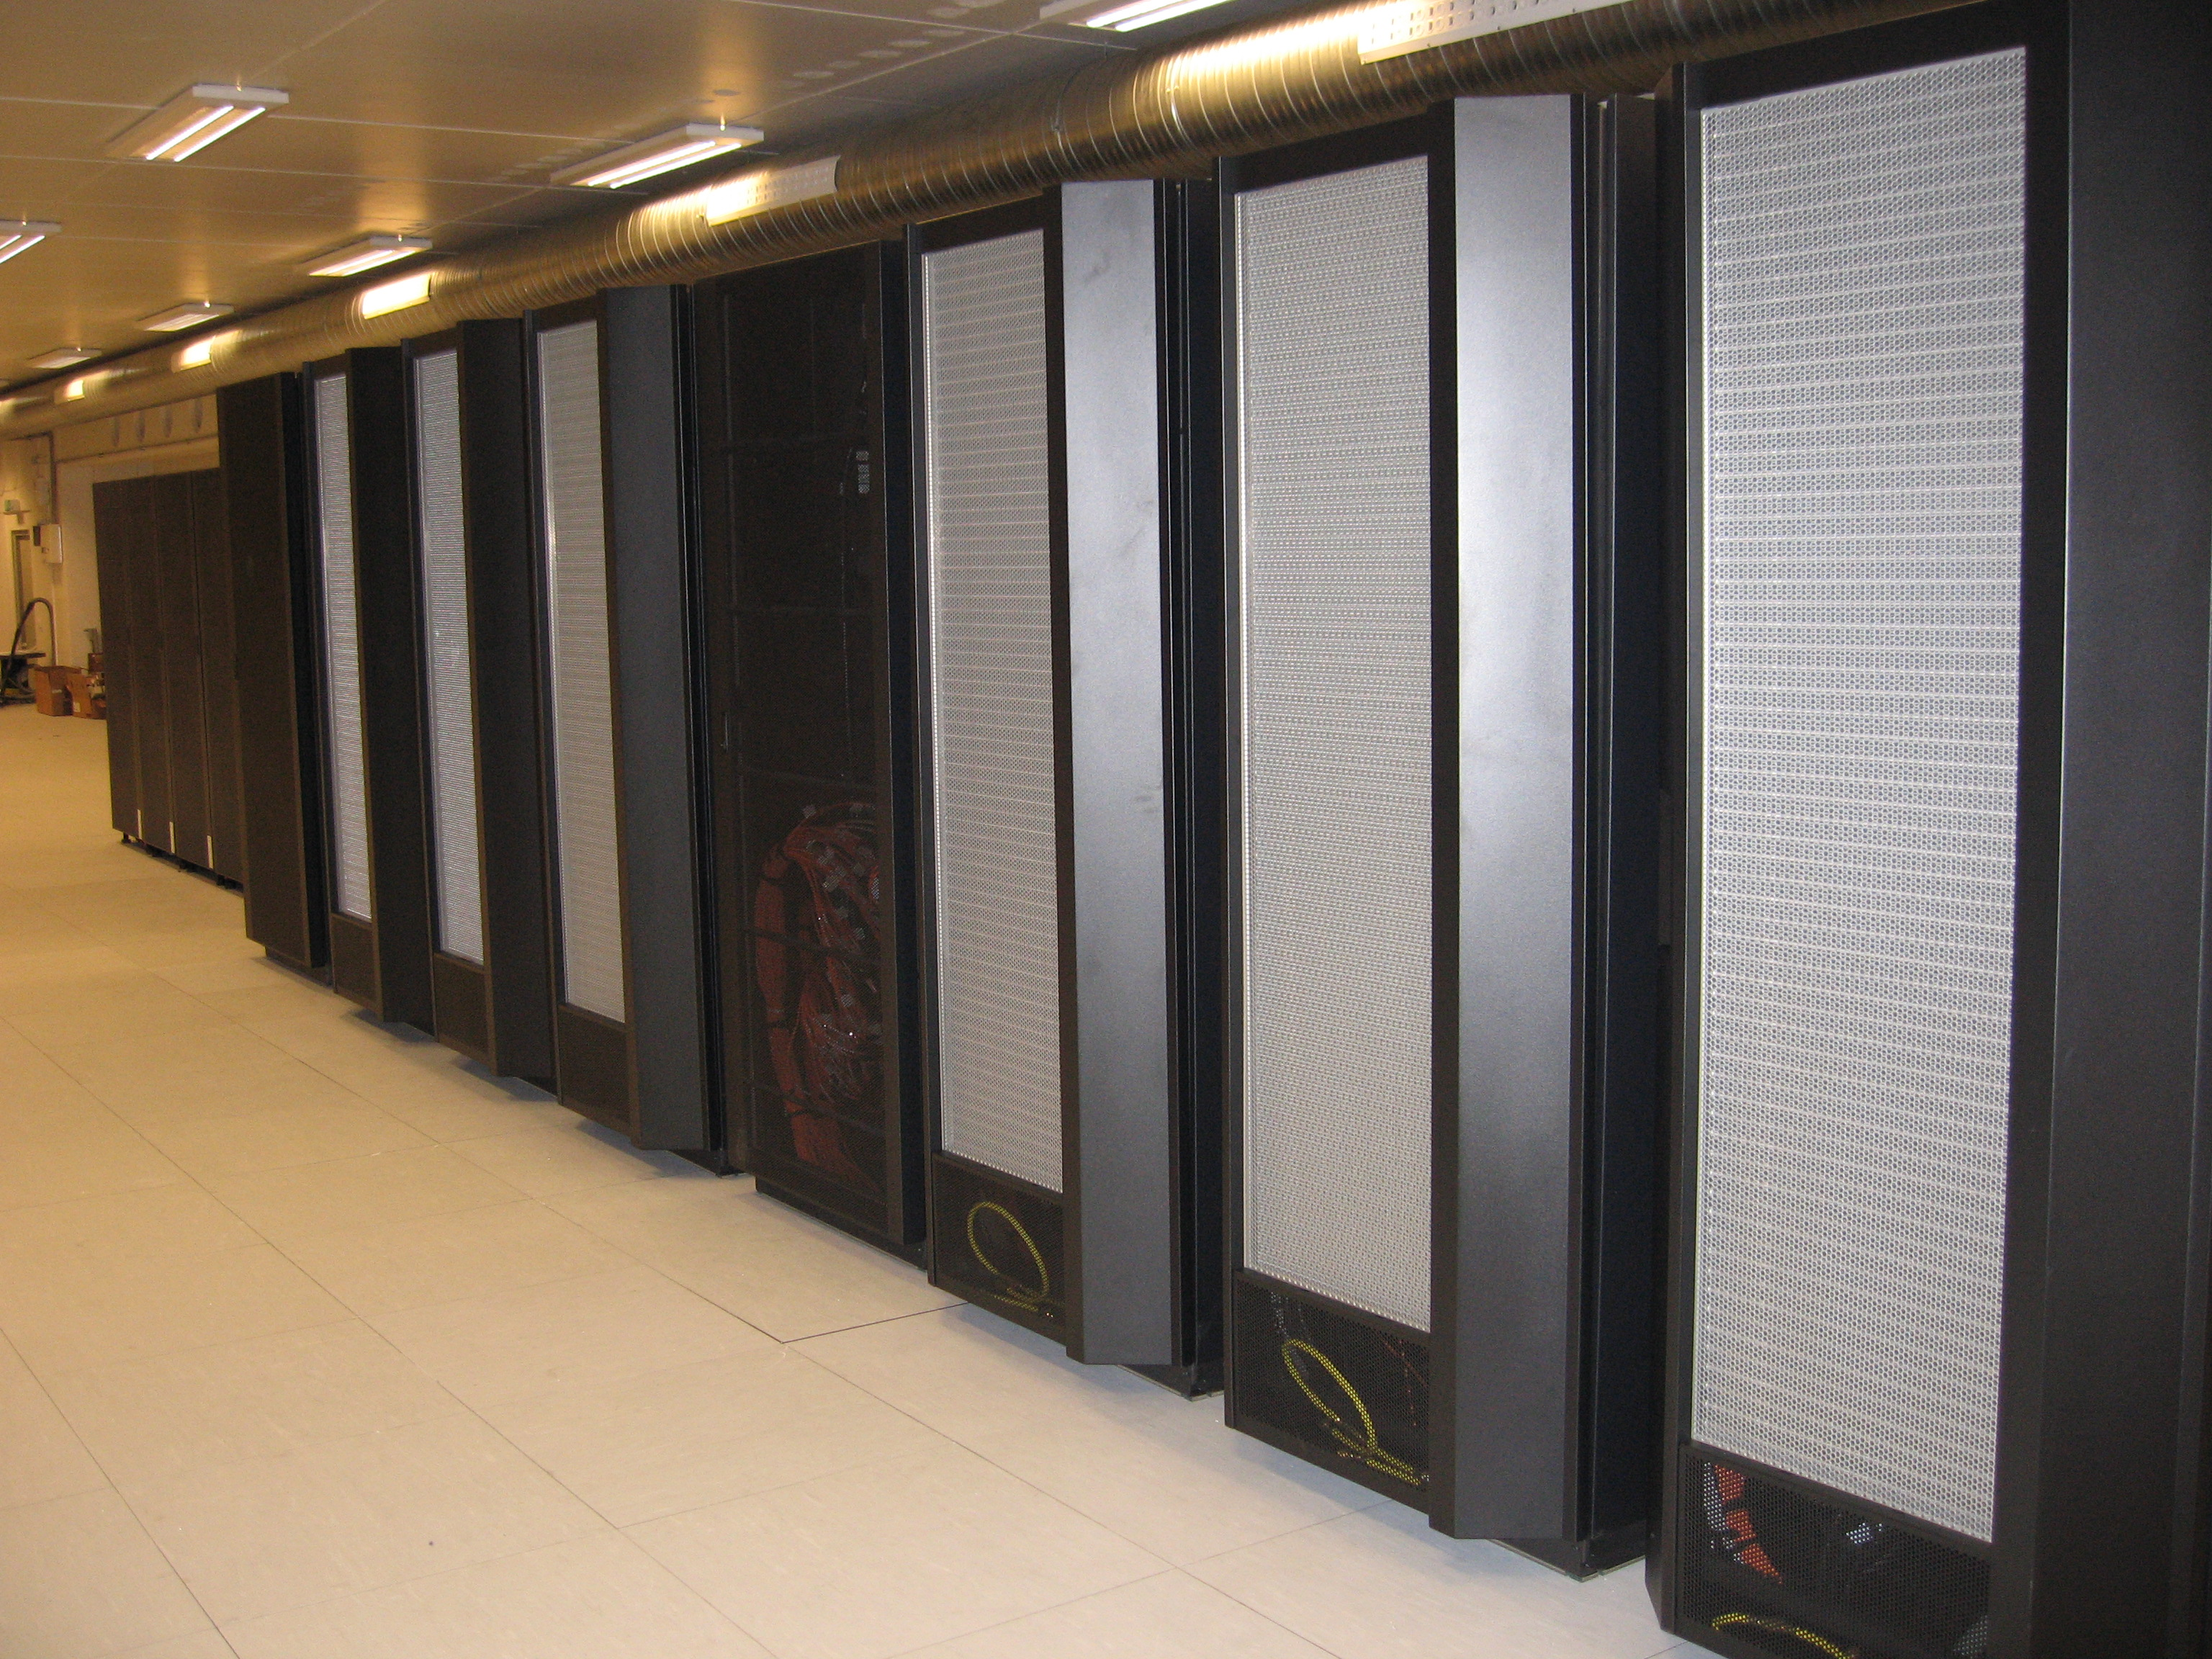
\includegraphics[height=0.6\textheight]{njord_2} \\
    \emph{Njord}: 3000 processors.
  \end{center}
\end{frame}

\begin{frame}
  \frametitle{Current supercomputer at NTNU}
  \begin{center}
    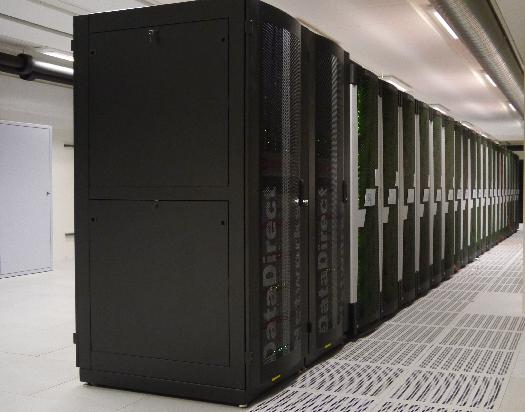
\includegraphics[height=0.6\textheight]{vilje} \\
    \emph{Vilje}: 22500 processors.
  \end{center}
\end{frame}

\begin{frame}
  \frametitle{Current supercomputer at NTNU}
  \begin{itemize}
  \item Full name: \texttt{vilje.hpc.ntnu.no}
  \item System: SGI Altix ICE
  \item Type: Distributed SMP
  \item Nodes: 1404
  \item Each node is a shared memory system with two octa-core chips and
    $\SI{32}{\giga\byte}$ memory.
  \item Physical cores: 22464
  \item Logical cores: 44928
  \item CPU: Intel Xeon (Sandy Bridge)
  \item Theoretical peak performance: $\SI{479.23}{\tera\flop}$
  \end{itemize}
\end{frame}

\begin{frame}
  \frametitle{Example: weather forecasting}
  \begin{center}
    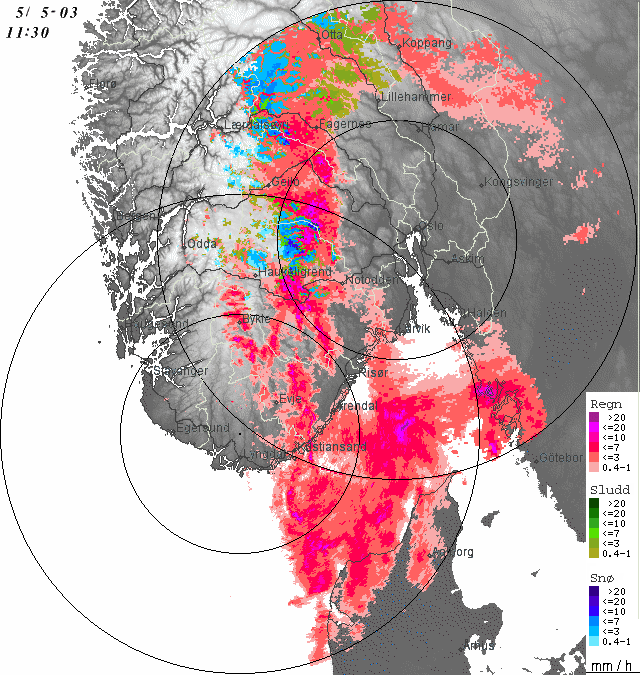
\includegraphics[height=0.7\textheight]{met} \\
    For more information, see \url{http://met.no}
  \end{center}
\end{frame}

\begin{frame}
  \frametitle{Example: climate modelling}
  \begin{center}
    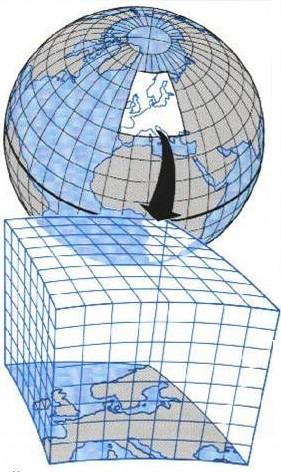
\includegraphics[height=0.7\textheight]{climate_model} \\
    For more information, see \url{http://www.bjerknes.uib.no}
  \end{center}
\end{frame}

\end{document}

